\newpage
\section{Externalidades}

Al abordar la temática de externalidades saldremos del marco Walrasiano anterior y volvemos a los modelos de Equilibrio Parcial. Las externalidades es uno de los problemas canónicos que aborda la economía, las posibles soluciones tienen ciertos tintes ideológicos según se le de más poder a lo privado o lo público.

Consideramos como externalidad la situación donde, ya sea la producción o consumo de un bien, tiene efectos en el bienestar de un tercero que no participa del mercado. Entre tantos ejemplos típicos encontramos las externalidades ambientales, el caso del fumador, la educación, entre otros.

\subsection{Externalidad en la producción}

Para analizar el funcionamiento de las externalidades negativas en la producción, utilizaremos como benchmark el equilibrio parcial de un mercado en competencia perfecta. Este modelo de mercado se compone por una oferta y demanda privada, las cuales en su interacción nos entregan un precio y una cantidad de equilibrio.

La oferta privada en este mercado está definida por el costo marginal de producción del bien ($Cmg$) percibidos por quien produce, estos pueden ser costos provenientes de la compra de insumos, gastos en energía, arriendo de un local, etc. 

\begin{figure}[htbp]
    \centering
    \caption{Equilibrio parcial en competencia perfecta}
    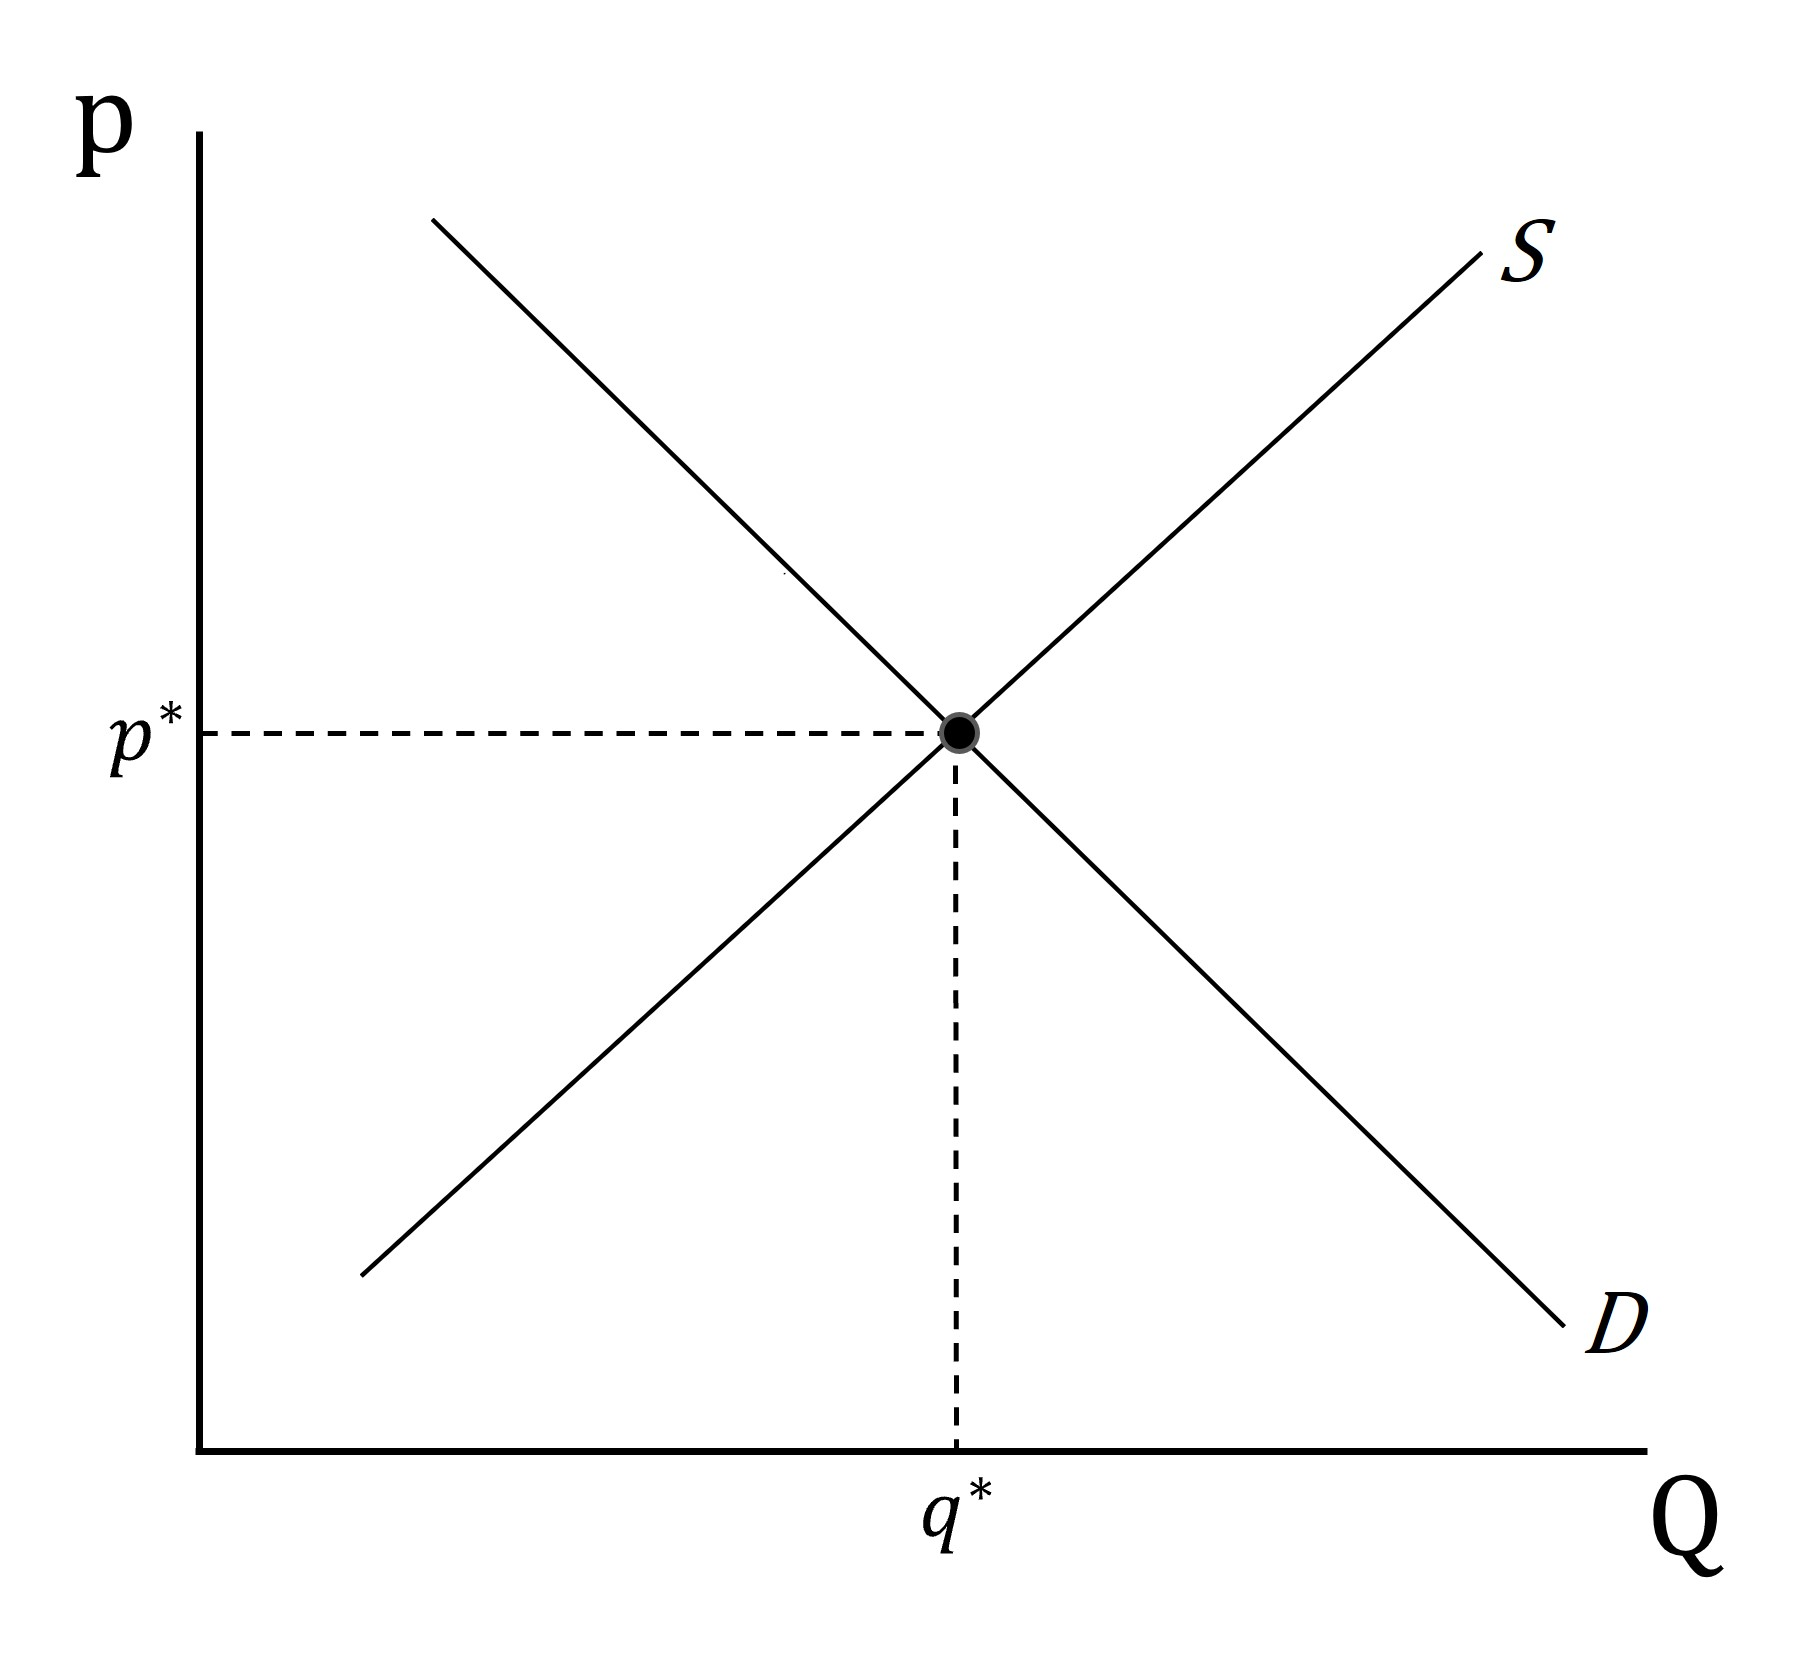
\includegraphics[width=0.5\textwidth]{Figuras/Eq Parcial EXT.jpg}
    \label{fig:Eq parcial}
\end{figure}

Para añadir externalidades negativas a este modelo, debemos considerar que existen costos adicionales que no son percibidos ni reconocidos por quién produce, por lo tanto tampoco son reflejados en la curva de oferta privada, estos nuevos costos los llamaremos ``costos sociales''. Con estos mayores costos, obtenemos que en equilibrio deberíamos observar un precio mayor y una cantidad producida menor.

\begin{figure}[htbp]
    \centering
    \caption{Externalidad en la producción}
    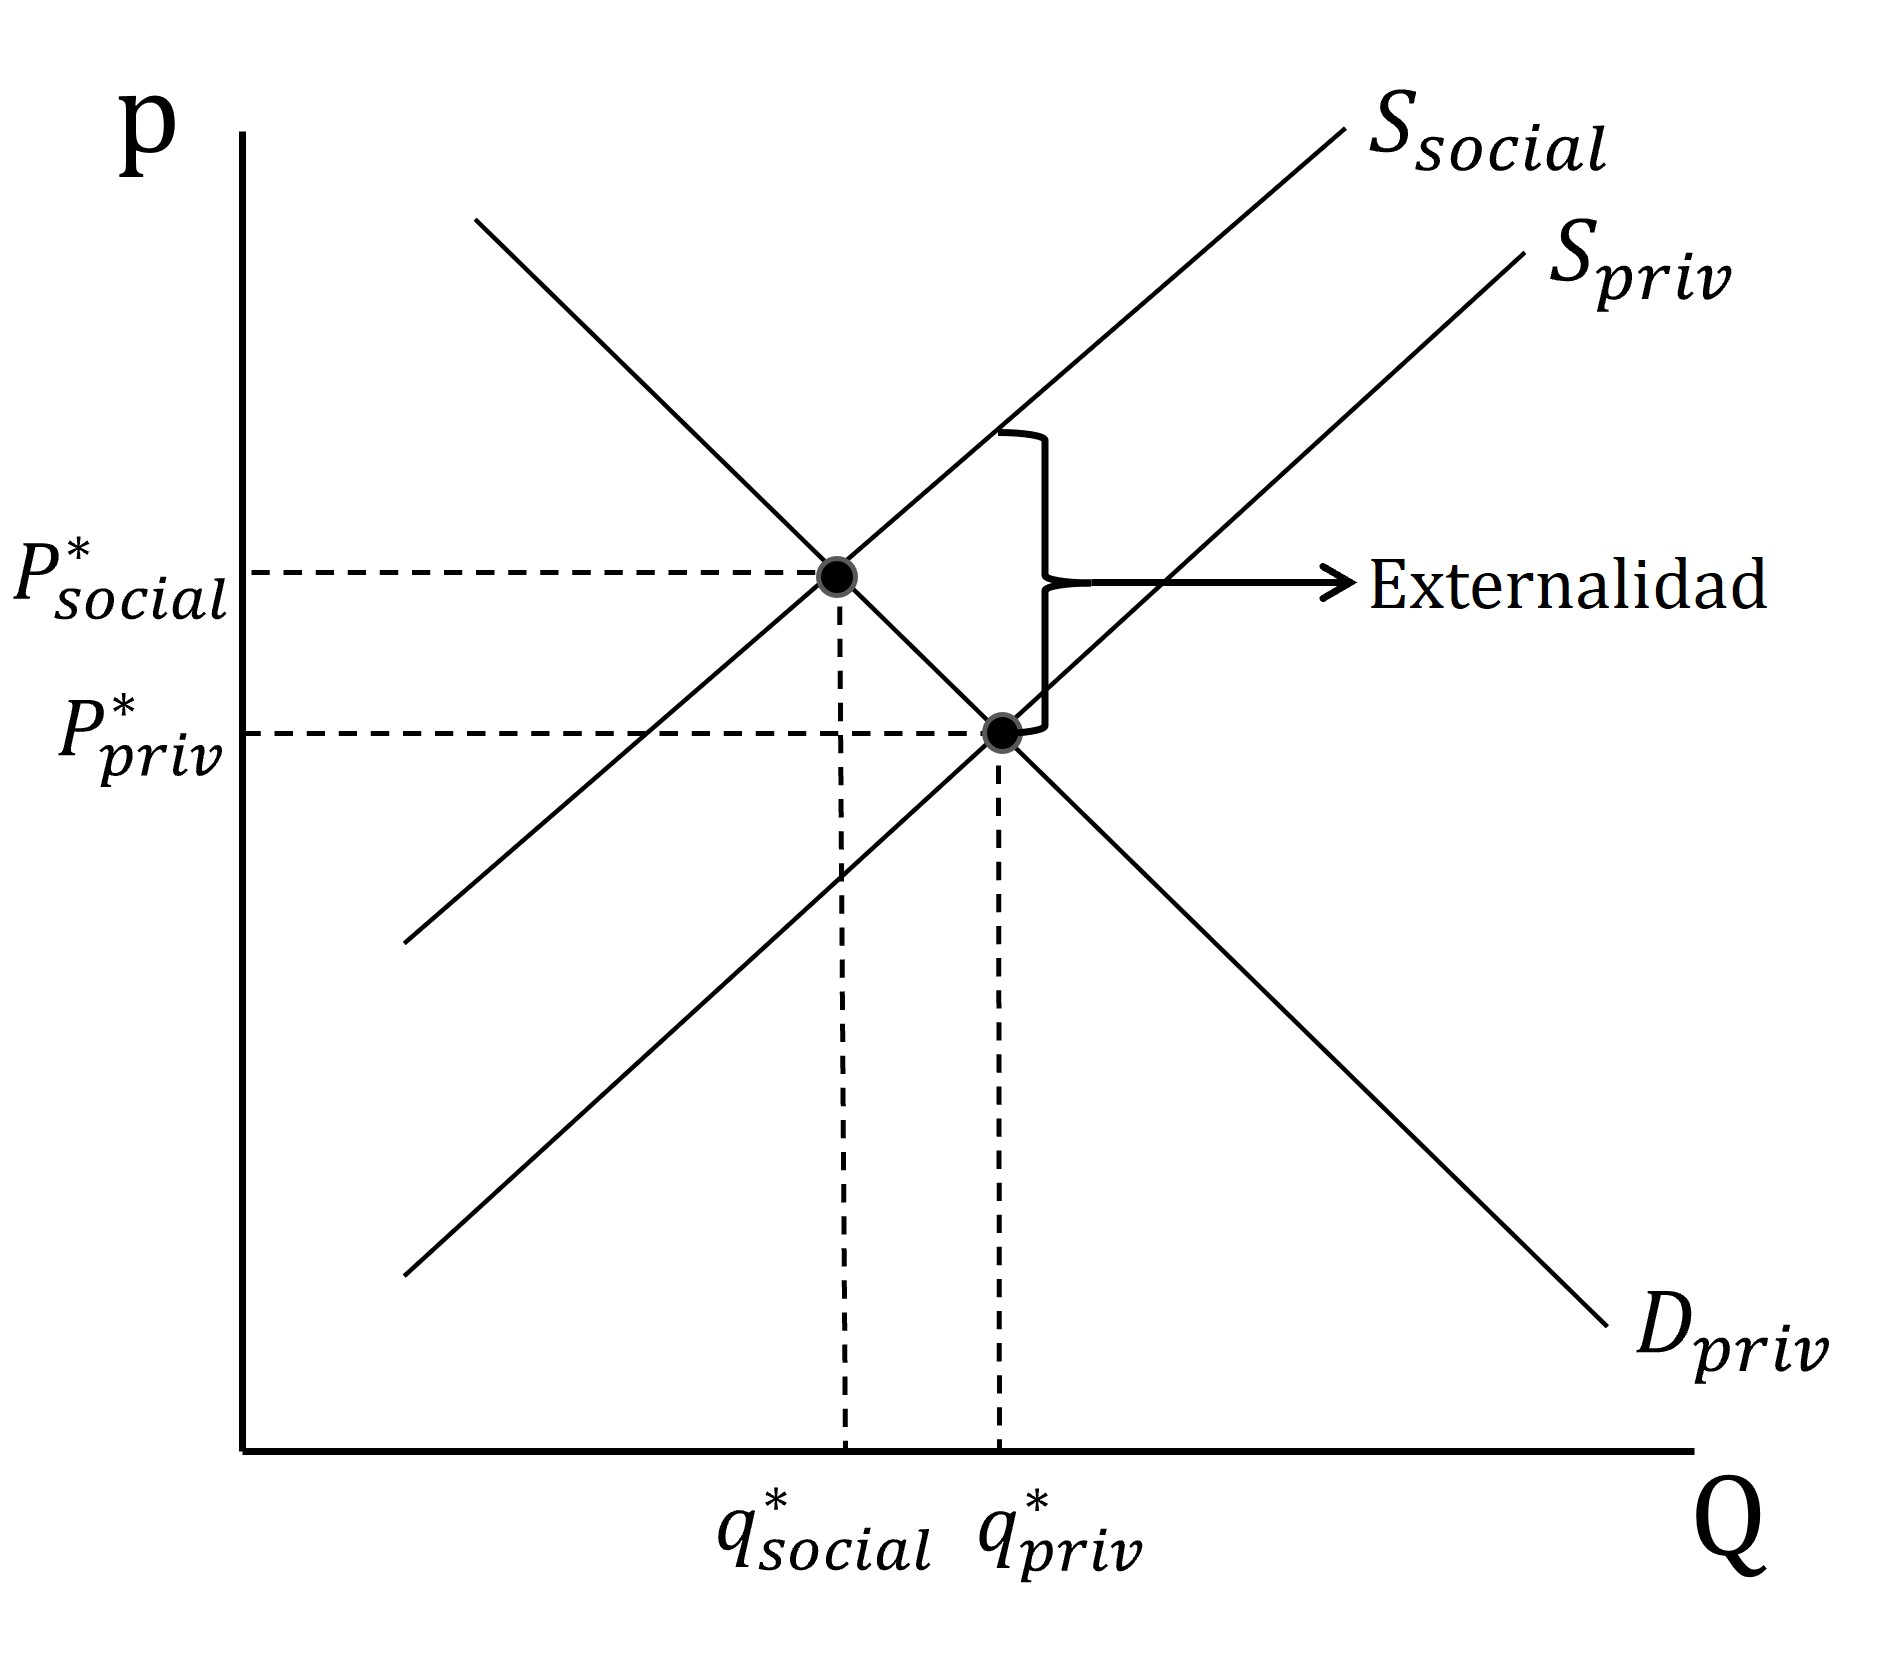
\includegraphics[width=0.5\textwidth]{Figuras/Externalidad Produccion.jpg}
    \label{fig:Ext. Producción}
\end{figure}

\subsubsection{Externalidad en la demanda}

Para el caso de externalidades positivas el problema no radica en costos no considerados, sino que existe una demanda social que es mayor a la privada. Para analizar este tipo de externalidad nuevamente utilizaremos como benchmark el equilibrio parcial de un mercado en competencia perfecta.

Con lo anterior tenemos que la demanda privada representa la disposición a pagar por el consumo individual de un bien, esto genera que se subestimen los beneficios que tiene sobre la sociedad el consumo de dicho bien. Por otro lado, la demanda social si refleja de manera fidedigna los beneficios generados a nivel social por el consumo del bien, la internalización de estos beneficios resultaría en una mayor disposición a pagar.

El resultado del equilibrio en el mercado considerando la demanda social nos entrega un mayor precio y cantidad producida.

Las externalidades negativas tambien se pueden representar por el lado de la demanda, esto ocurre cuando el efecto en el bienestar del tercero viene dado por el consumo del bien más que por su producción, ejemplo de esto es el consumo del cigarro, con esto tenemos que quien consume no internaliza la desutilidad que genera en los demás agentes y por lo tanto no representa la disposición a pagar de la sociedad. El equilibrio del mercado resulta diferente para este caso, ya que tenemos que en equilibrio el precio y la cantidad producida disminuyen

\subsubsection{Solución Pública}

La solución de carácter pública para corregir esta falla de mercado fue creada por el economista \textbf{Arthur Pigou}\marginnote{\textbf{Arthur Pigou:}(1877-1959) Economista inglés de la Universidad de Cambridge, conocido por inventar el término \textit{externalidades} y contribuir con su solución pública.}, los mecanismos utilizados por esta solución los conocemos como \textit{impuestos y subsidios pigouvianos}, y los supuestos utilizados son que el estado tiene información completa acerca de las preferencias de la sociedad y además la capacidad suficiente para que sus impuestos o subsidios modifiquen el comportamiento de los agentes.

Es importante conocer la diferencia entre tipo de impuestos, de manera general en el estado encontramos impuestos utilizados con el fin de recaudar y subsidios que se enfocan en redistribuir, por otra parte tenemos los impuestos y subsidios pigouvianos que corrigen externalidades mediante un cambio en el comportamiento de los agentes. Dentro de los ejemplos clásicos de impuestos y subsidios pigouvianos encontramos el impuesto al tabaco y los colegios subvencionados.

\subsubsection{Medida de efectividad}

Para poder medir la efectividad de la solución pública utilizaremos como herramienta la \textit{evaluación social de proyectos públicos}, esta es un área de la economía desarrollada por \textbf{Arnold Harberger}\marginnote{\textbf{Arnold Harberger:}(1924-) Economista estadounidense de la Universidad de Chicago, conocido por ser pionero en el estudio de la evaluación social de proyectos públicos}. Considerando que la aplicación de impuestos o subsidios es costosa (Ej: costos de administración), la evaluación social consiste en comparar las preferencias sociales y privadas, para determinar la magnitud de la \textit{pérdida social}\footnote{En inglés se conoce como \textit{dead weight loss (DWL)}} existente en un mercado, representada gráficamente por los \textit{triángulos de Harberger}, con esto podremos comparar los costos y beneficios de resolver una externalidad y usar esto como medida de eficiencia. 